\documentclass{beamer}
	\setbeamertemplate{navigation symbols}{} %para no pintar los iconos abajo a la derecha
	\setbeamersize{text margin left=5mm,text margin right=5mm} 

\usepackage[spanish]{babel}
\usepackage{tikz-cd}
\usepackage{listings}
%\usecolortheme{dove}
\usepackage{xcolor}
	\definecolor{RojoNebrija}{RGB}{194,0,47}
	\definecolor{GrisNebrija1}{RGB}{127,127,127}
	\definecolor{GrisNebrija2}{RGB}{166,166,166}
	\definecolor{GrisNebrija3}{RGB}{191,191,191}
	
\usecolortheme[named=RojoNebrija]{structure}

		
\title{DESARROLLO DE UNA APLICACIÓN WEB Y ESTUDIO PRÁCTICO DE HERRAMIENTAS PARA EL DESPLIEGUE DE SU INFRAESTRUCTURA COMO CÓDIGO}
\subtitle{\color{black}{Prácticas en Empresa I}}
\author{Óscar Salvador}

\usefonttheme{serif}

\begin{document}
	\frame {
		\titlepage
	}

%	\frame{
%		\frametitle{Introducción}
%		%\framesubtitle{GlusterFs}
%		\begin{itemize}
%		\footnotesize
%			\item[] Definición: Base de datos cuyos contenidos estan modelados con cualquier método salvo tablas relacionales \footnote{\tiny{documentacion/paralelo2serie/4/timing\_p2s\_4.rpx}}
%			\linebreak
%		\end{itemize}		

%		\centering
%		\resizebox{0.2\textwidth}{!}{%
%			\includegraphics[width=\textwidth]{glusterfs.png}
%		}
%	}
	
	\frame{
		\frametitle{Introducción}
			\begin{itemize}
				\footnotesize
				\item[] \textbf{Infraestructura}: HW y SW necesarios para sostener una aplicación
				\linebreak
			
				\item[] \textbf{Infraestructura como Código}: control de versión, pipelines
				\linebreak
				
				\item[] Herramientas para \textit{IaC}: \textbf{Terraform} y \textbf{Ansible}
				\linebreak
				
				\item[] Lenguajes \textbf{declarativos}: \underline{que} quieres, no como conseguirlo
				\linebreak
			\end{itemize}

	}
	
	\frame{
		\frametitle{Aplicación Web}

			
			\begin{figure}[htb]
				\centering
				\resizebox{.9\linewidth}{!}{%
					\includegraphics{../drawio/general2.drawio.pdf}
				}
			\end{figure}

	}
	

	\frame{
		\frametitle{Requisitos de infraestructura}
			\begin{figure}[htb]
				\centering
				\resizebox{.85\linewidth}{!}{%
					\includegraphics{../drawio/general-infra.drawio.pdf}
				}
			\end{figure}
	}



% dos cosas lo hacen especiales, tfstate, captura (que solo es un json) y grafo de dependencias


% los dos usan wrappers al rededor del api


	\frame{
		\frametitle{Uso de wrappers}
		\framesubtitle{\color{black}{Abstracción del API de la plataforma}}
		\begin{itemize}
		\footnotesize
			\item[] Terraform Core y Ansible Core
			\linebreak
		
			\item[] Terraform \textbf{providers}
			\linebreak
			
			\item[] Ansible \textbf{collections}
			\linebreak
		\end{itemize}
	}
	
	
	\frame{
		\frametitle{Terraform}
		\framesubtitle{\color{black}{Introducción}}
		\begin{itemize}
		\footnotesize
			\item[] Ficheros \textit{HCL}: Hashicorp Configuration Language, extensión \texttt{.tf}
			\linebreak
			
			\item[] Organización sencilla, orientado a polyrepo
			\linebreak
			
			\item[] Bloques principales: \texttt{provider}, \texttt{variable}, \texttt{data}, \texttt{resource} y \texttt{output}\footnote{\tiny{Sintaxis de referencia, documentación de Terraform [1]}}
			\linebreak
			
		\end{itemize}
	
			\begin{figure}[htb]
				\tiny
				\hspace{-1.5cm}
				\texttt{<BLOCK TYPE>\ '<BLOCK LABEL>' '<BLOCK LABEL>' \{} 
				
				\hspace{-4cm}
				\texttt{\color{gray}{\# Block body}}
				
				\hspace{-1cm}
				\texttt{<IDENTIFIER>\ =\ <EXPRESSION>\ \color{gray}{\# Argument}} 

				\hspace{-6.5cm}		
				\texttt{\}}
			\end{figure}
	}
	
	
	
	\frame{
		\frametitle{Terraform}
		\framesubtitle{\color{black}{Funcionamiento}}
		\begin{itemize}
		\footnotesize
			\item[] Fichero \texttt{terraform.tfstate}
			\linebreak
		
			\item[] Construcción del \textit{grafo de dependencias}
			\linebreak
			
		\end{itemize}
		
			\begin{figure}[htb]
				\centering
				\resizebox{.8\linewidth}{!}{%
					\includegraphics{../terraform-graph/base-graph.pdf}
				}
			\end{figure}
			
	}
	
	
	
	\frame{
		\frametitle{Terraform}
		\framesubtitle{\color{black}{Extracto del grafo de dependencias del frontend}}

			\begin{figure}[htb]
				\centering
				\resizebox{.8\linewidth}{!}{%
					\includegraphics{../terraform-graph/demo-graph.pdf}
				}
			\end{figure}
			
	}
	
	
	\frame{
		\frametitle{Terraform}
		\framesubtitle{\color{black}{Implementación}}

			\begin{itemize}
				\footnotesize
				\item[] Diseño en tres partes, proyectos de Terraform inconexos
				\linebreak

				\item[] Terraform solo aprovisiona, no puede construir imágenes Docker
				\linebreak
	
			\end{itemize}
			
			\begin{figure}[htb]
				\centering
				\resizebox{.7\linewidth}{!}{%
					\includegraphics{../drawio/general2-resueltos.drawio.pdf}
				}
			\end{figure}
	}
	
	\frame{
		\frametitle{Terraform}
		\framesubtitle{\color{black}{Implementación}}
			
			\begin{figure}[htb]
				\centering
				\resizebox{.9\linewidth}{!}{%
					\includegraphics{../drawio/terraform-etapas.drawio.pdf}
				}
			\end{figure}
	}
	
	
	
	\frame{
		\frametitle{Ansible}
		\framesubtitle{\color{black}{Introducción}}
		\begin{itemize}
		\footnotesize
			\item[] Ficheros \textit{YAML} organizados en roles, y estos en playbooks
			\linebreak
			
			\item[] Organización escalable, un playbook \underline{es} un pipeline, portabilidad
			\linebreak
			
			\item[] Fichero ``play'' en el que se organizan los roles
			\linebreak
			
		\end{itemize}
	
		\begin{columns}[T] % align columns
		\begin{column}{.48\textwidth}
		
			\begin{figure}
        \tiny
        
        \texttt{playbook} 
        
            \hspace{.5cm}
            \texttt{inventory} 
        
                \hspace{.6cm}
                \texttt{hosts}
        
            \hspace{.2cm}
            \texttt{roles}
        
                \hspace{.7cm}
                \texttt{role-1}
            
                \hspace{.5cm}
                \texttt{ ... }
        
                \hspace{.7cm}
                \texttt{role-N}
        
                    \hspace{1cm}
                    \texttt{files}
    
                    \hspace{1.35cm}
                    \texttt{handlers}
    
                    \hspace{.9cm}
                    \texttt{meta}
    
                    \hspace{1cm}
                    \texttt{tasks}
    
                        \hspace{1.8cm}
                        \texttt{main.yml}    
    
                    \hspace{1.5cm}
                    \texttt{templates}
    
                    \hspace{.95cm}
                    \texttt{vars}                
                    
            \hspace{.2cm}
            \texttt{play} 
    	\end{figure}
		\end{column}%
		\hspace{-3cm}
		\begin{column}{.48\textwidth}
			\begin{figure}
					\tiny
					\hspace{-1cm}
          \texttt{- name: <Nombre del play>} 
      
          \hspace{.1cm}
          \texttt{host: <Nodo gestionado destino>} 
      
          \hspace{.0cm}
          \texttt{connection: <Tipo de conexion>}
      
          \hspace{-1.55cm}
          \texttt{strategy: <Tipo>}
          
          \hspace{-2.65cm}
          \texttt{roles:}
      
              \hspace{.65cm}
              \texttt{- role1: <Nombre de la carpeta>}
      
              \hspace{-1.45cm}
              \texttt{tags: []}
      
              \hspace{.65cm}
              \texttt{- role2: <Nombre de la carpeta>}
      
              \hspace{-1.45cm}
              \texttt{tags: []}
			\end{figure}
		\end{column}%
		
		\end{columns}		
	}
	
	\frame{
		\frametitle{Ansible}
		\framesubtitle{\color{black}{Funcionamiento}}
		\begin{itemize}
		\footnotesize
			\item[] Declarativo a nivel de tarea
			\linebreak
			
			\item[] Conexión \textit{SSH} a cada host y ejecución de los comandos necesarios
			\linebreak
			
			\item[] Secuencial a nivel de play y de rol, asincronía para paralelizar
			\linebreak
			
			\item[] Funcionalidades como la concurrencia dependen del desarrollador
			\linebreak
			
		\end{itemize}
	
			\begin{figure}[htb]
				\tiny
        \hspace{0cm}
				\texttt{- name: <Nombre de la tarea>} 
            
        \hspace{-1.9cm}
        \texttt{modulo:} 
    
            \hspace{.7cm}
            \texttt{campo1\_del\_modulo: <valor>}
        
            \hspace{.7cm}
            \texttt{campo2\_del\_modulo: <valor>}
    
        \hspace{1.6cm}
        \texttt{register: <Nombre para los resultados>}    
        
        \hspace{2.15cm}
        \texttt{async: <Segundos antes de abortar la tarea>}    

        \hspace{2.15cm}
        \texttt{poll: <Segundos entre peticiones de estado>}    
			\end{figure}

	}
	
	
	\frame{
		\frametitle{Ansible}
		\framesubtitle{\color{black}{Implementación}}
			
			\begin{figure}[htb]
				\centering
				\resizebox{.88\linewidth}{!}{%
					\includegraphics{../drawio/parallel-ansible-etapas.drawio.pdf}
				}
			\end{figure}
	}
	
	
	\frame{
		\frametitle{Comparación}
		\framesubtitle{\color{black}{Rendimiento}}
		
			
			\begin{figure}[htb]
				\centering
				\resizebox{\linewidth}{!}{%
					\includegraphics{../charts/tiempos.pdf}
				}
			\end{figure}
	}
	
	
	\frame{
		\frametitle{Comparación}
		\framesubtitle{\color{black}{Verbosidad}}
		
			\begin{columns}[T] % align columns
		\begin{column}{.48\textwidth}
			\small Líneas de código
			\begin{figure}[htb]
				\centering
				\resizebox{\linewidth}{!}{%
					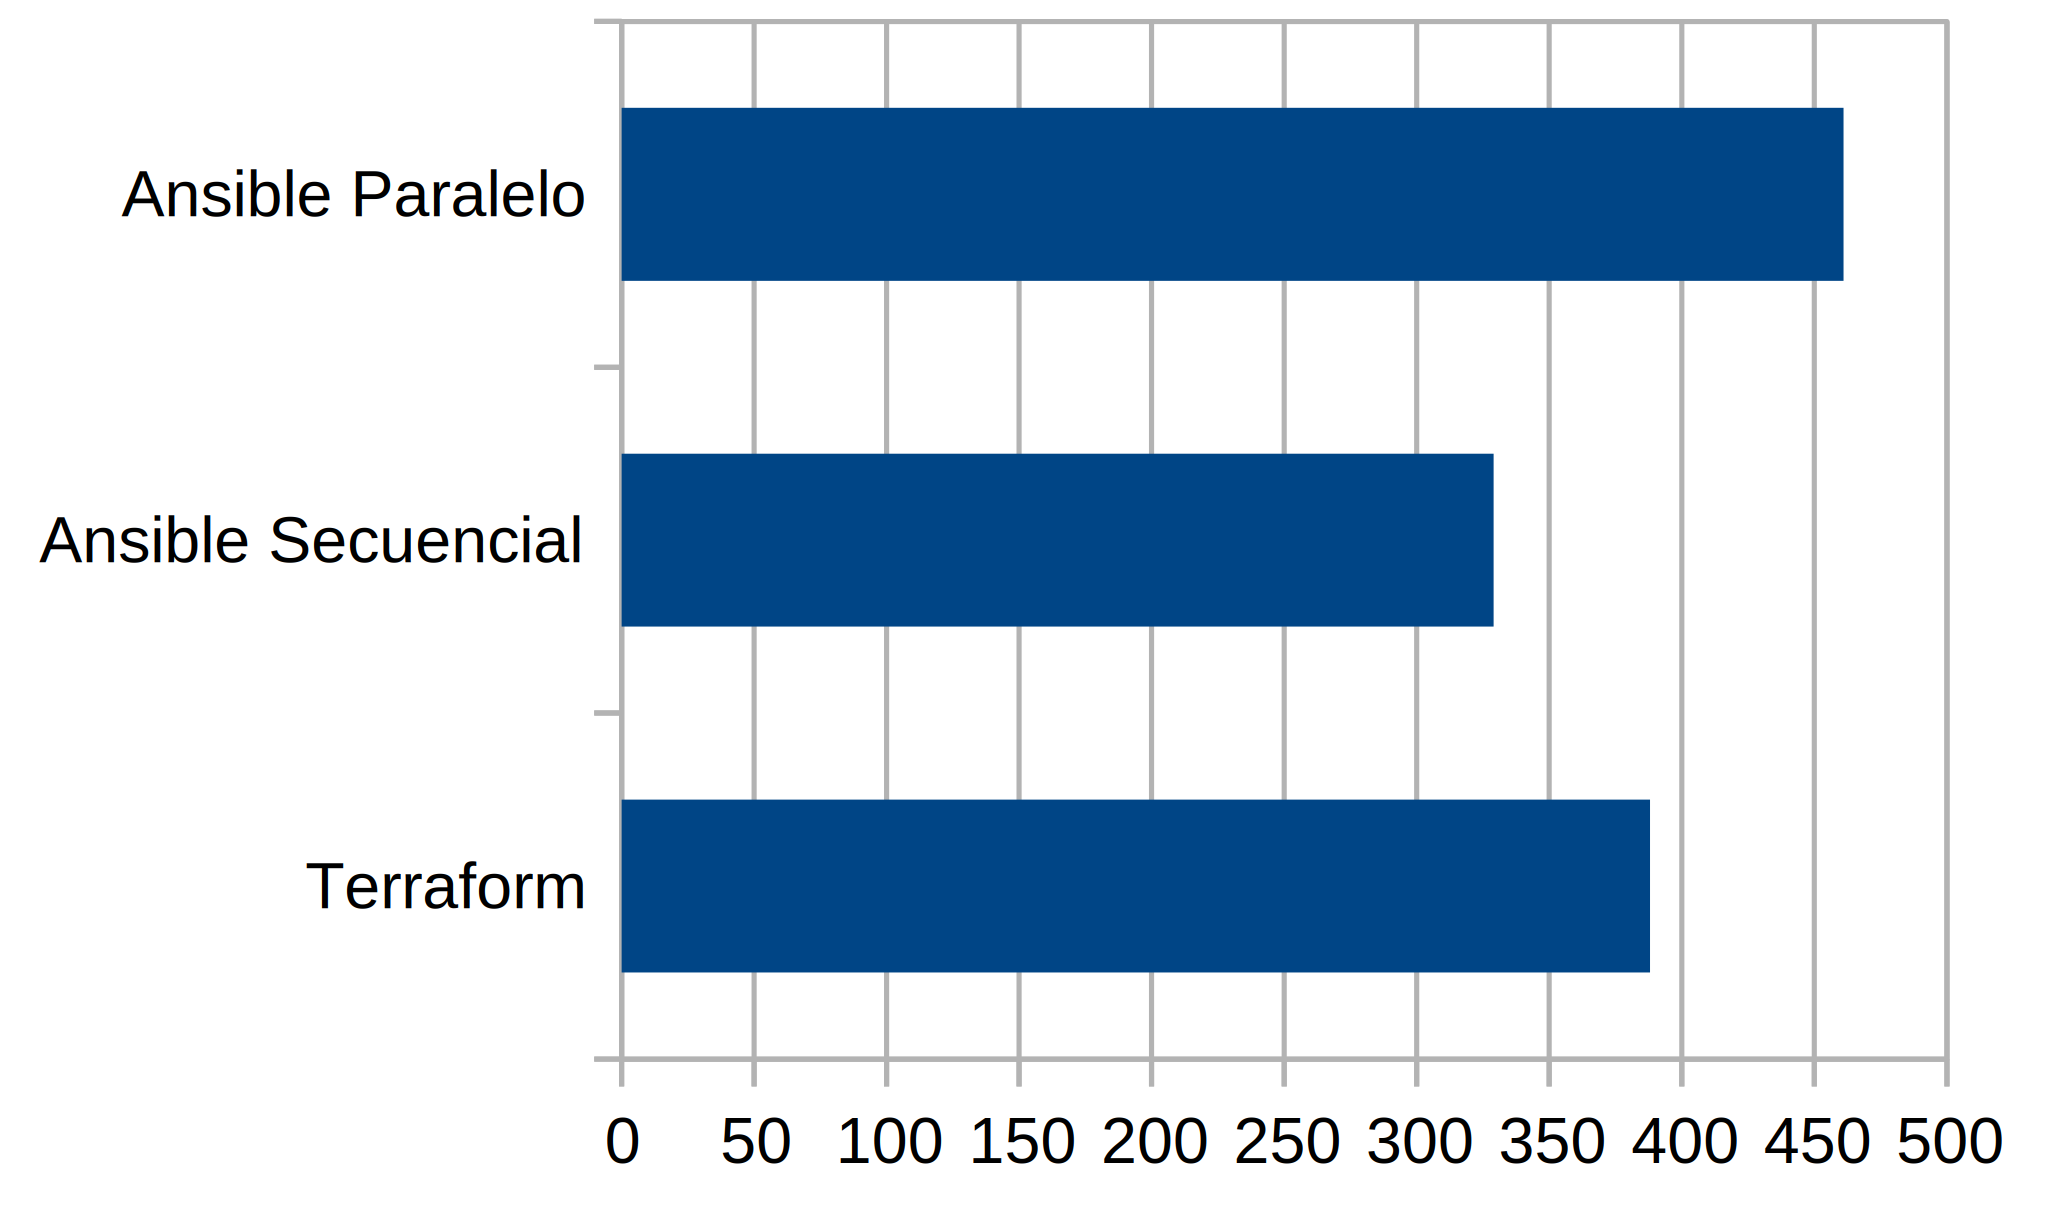
\includegraphics{../charts/lineas.pdf}
				}
			\end{figure}
			\end{column}%
		\hspace{0cm}
		\begin{column}{.48\textwidth}
			\small Caracteres
			\begin{figure}[htb]
				\centering
				\resizebox{.97\linewidth}{!}{%
					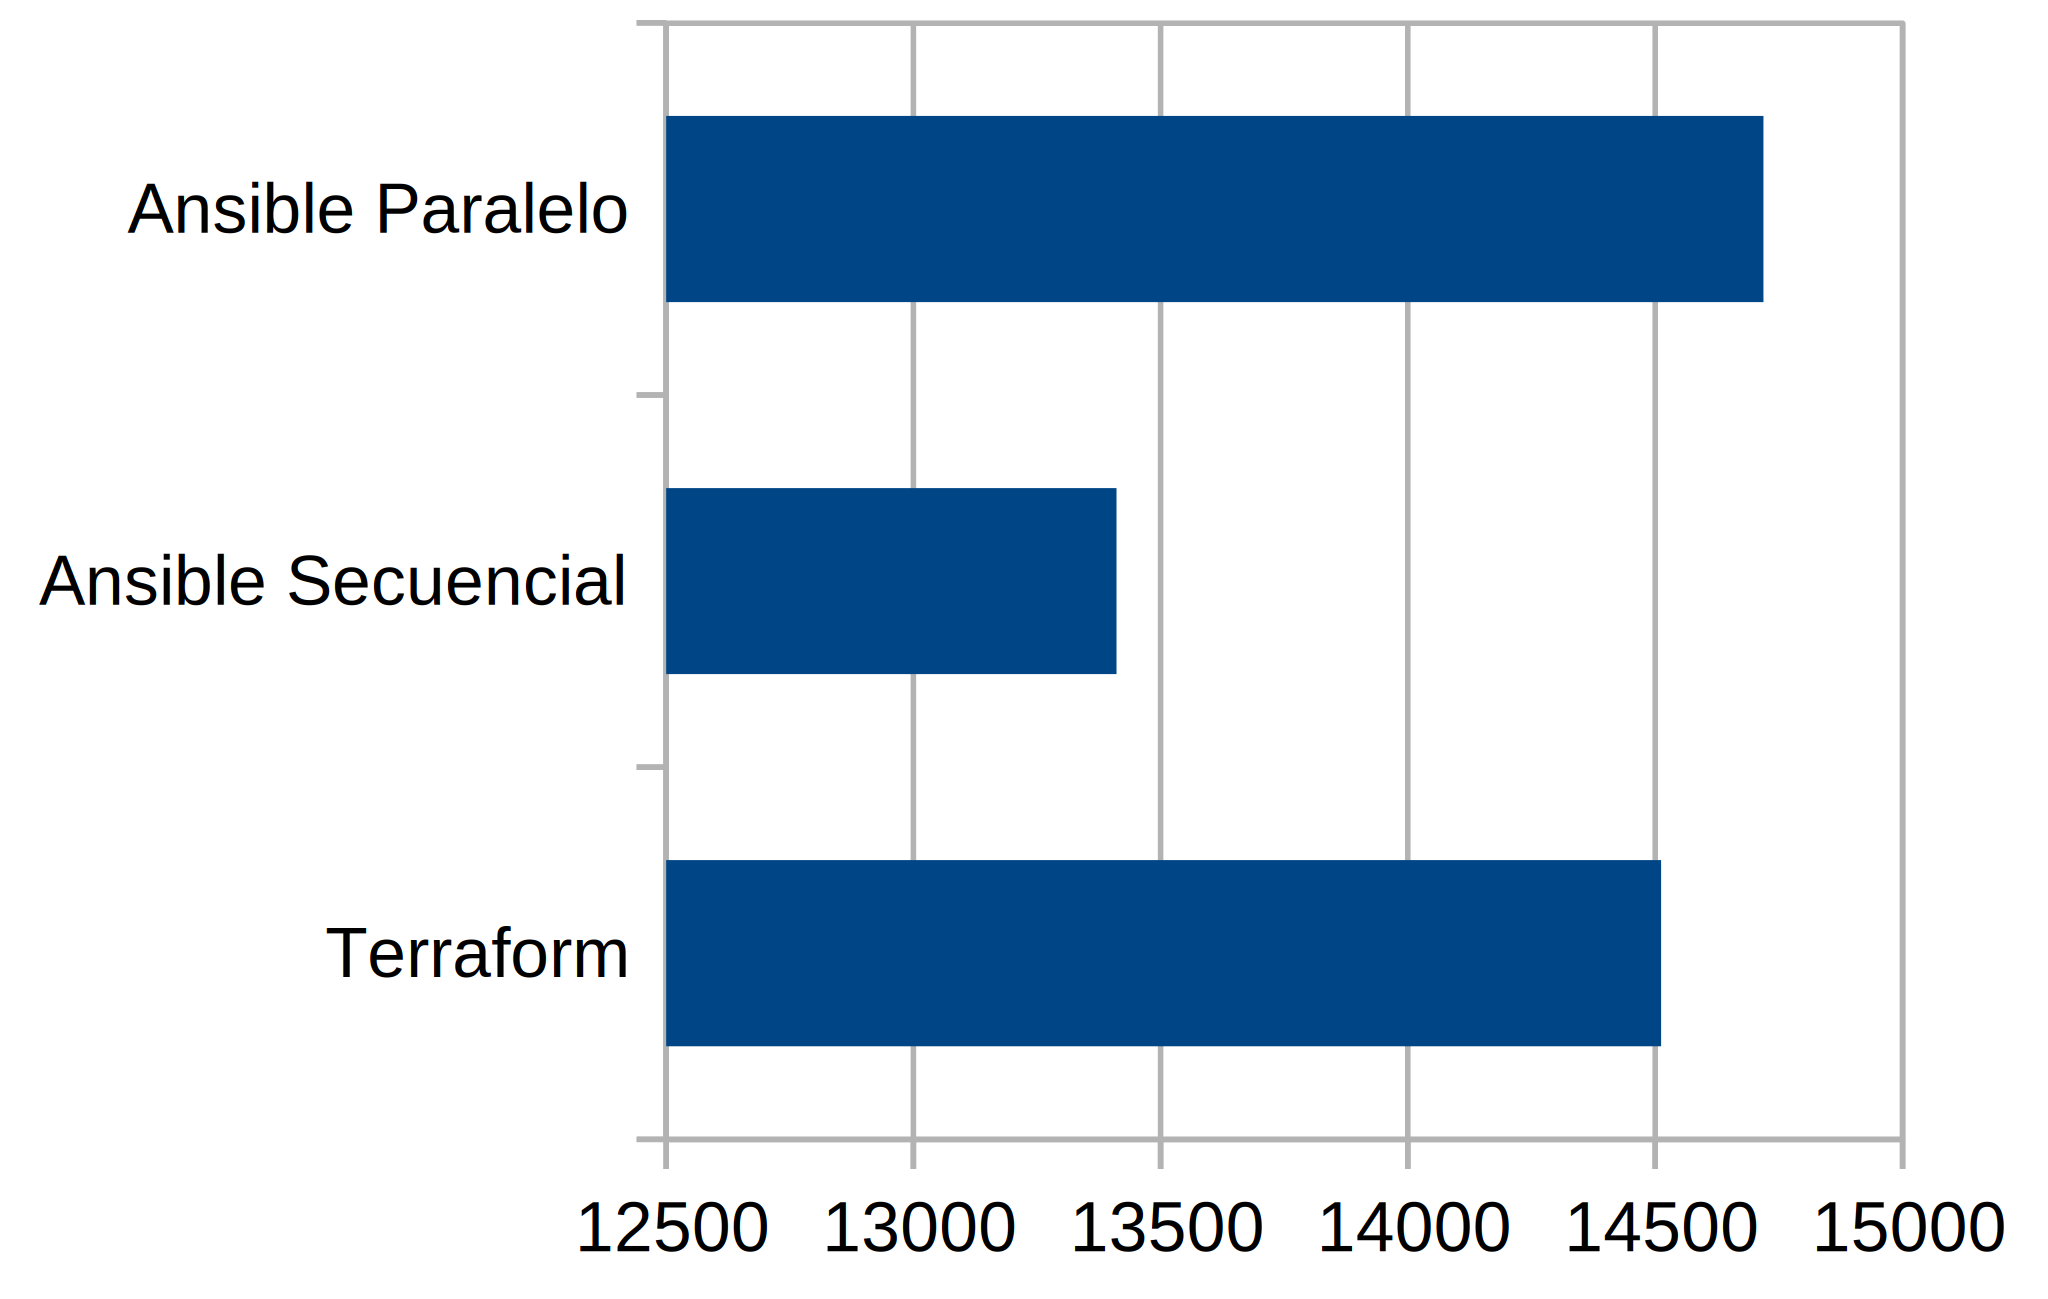
\includegraphics{../charts/caracteres.pdf}
				}
			\end{figure}
			\end{column}%
		
		\end{columns}		
	}
	
	
	
	
	\frame{
		\frametitle{Comparación}
		\framesubtitle{\color{black}{Relevancia}}
		\begin{itemize}
		\footnotesize			
			\item[] Sexta y séptima herramientas más populares en Stack Overflow\footnote{\tiny{Stack Overflow Survey 2022 § Desarrolladores Profesionales [2]}}
			\linebreak
			
		\end{itemize}
			
			\begin{figure}[htb]
				\centering
				\resizebox{.8\linewidth}{!}{%
					\includegraphics{../capturas/stack_overflow.png}
				}
			\end{figure}
	}
	
	
	\frame{
		\frametitle{Comparación}
		\framesubtitle{\color{black}{Relevancia, tendencia}}
		\begin{itemize}
		\footnotesize			
			\item[] Ligera pérdida de popularidad relativa de Ansible en Españafootnote\footnote{\tiny{Google Trends, Ansible, Terraform, últimos 5 años, en España [3]}}
			\linebreak
			
		\end{itemize}
			
			\begin{figure}[htb]
				\centering
				\resizebox{.9\linewidth}{!}{%
					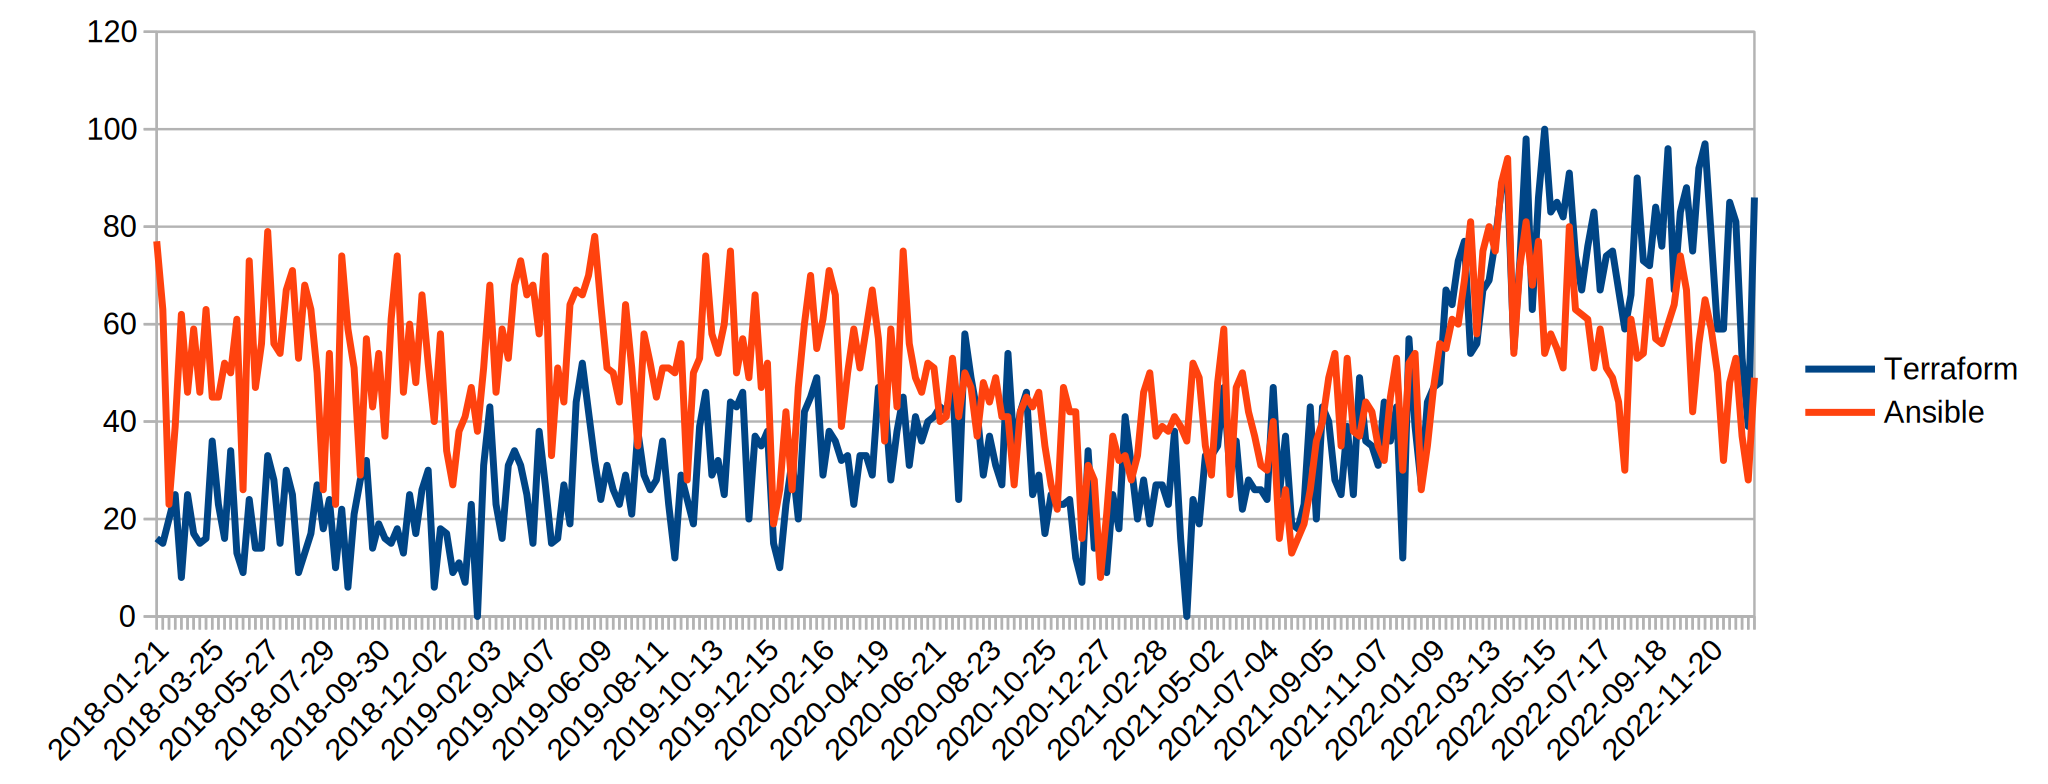
\includegraphics{../charts/trends-spanita.pdf}
				}
			\end{figure}
	}
	
	
	
	\frame{
		\frametitle{Comparación}
		\framesubtitle{\color{black}{Relevancia, tendencia}}
		\begin{itemize}
		\footnotesize			
			\item[] Aumento en demanda de Terraform a nivel mundial\footnote{\tiny{Google Trends, Ansible, Terraform, últimos 5 años, en el mundo [4]}}
			\linebreak
			
		\end{itemize}
			
			\begin{figure}[htb]
				\centering
				\resizebox{.9\linewidth}{!}{%
					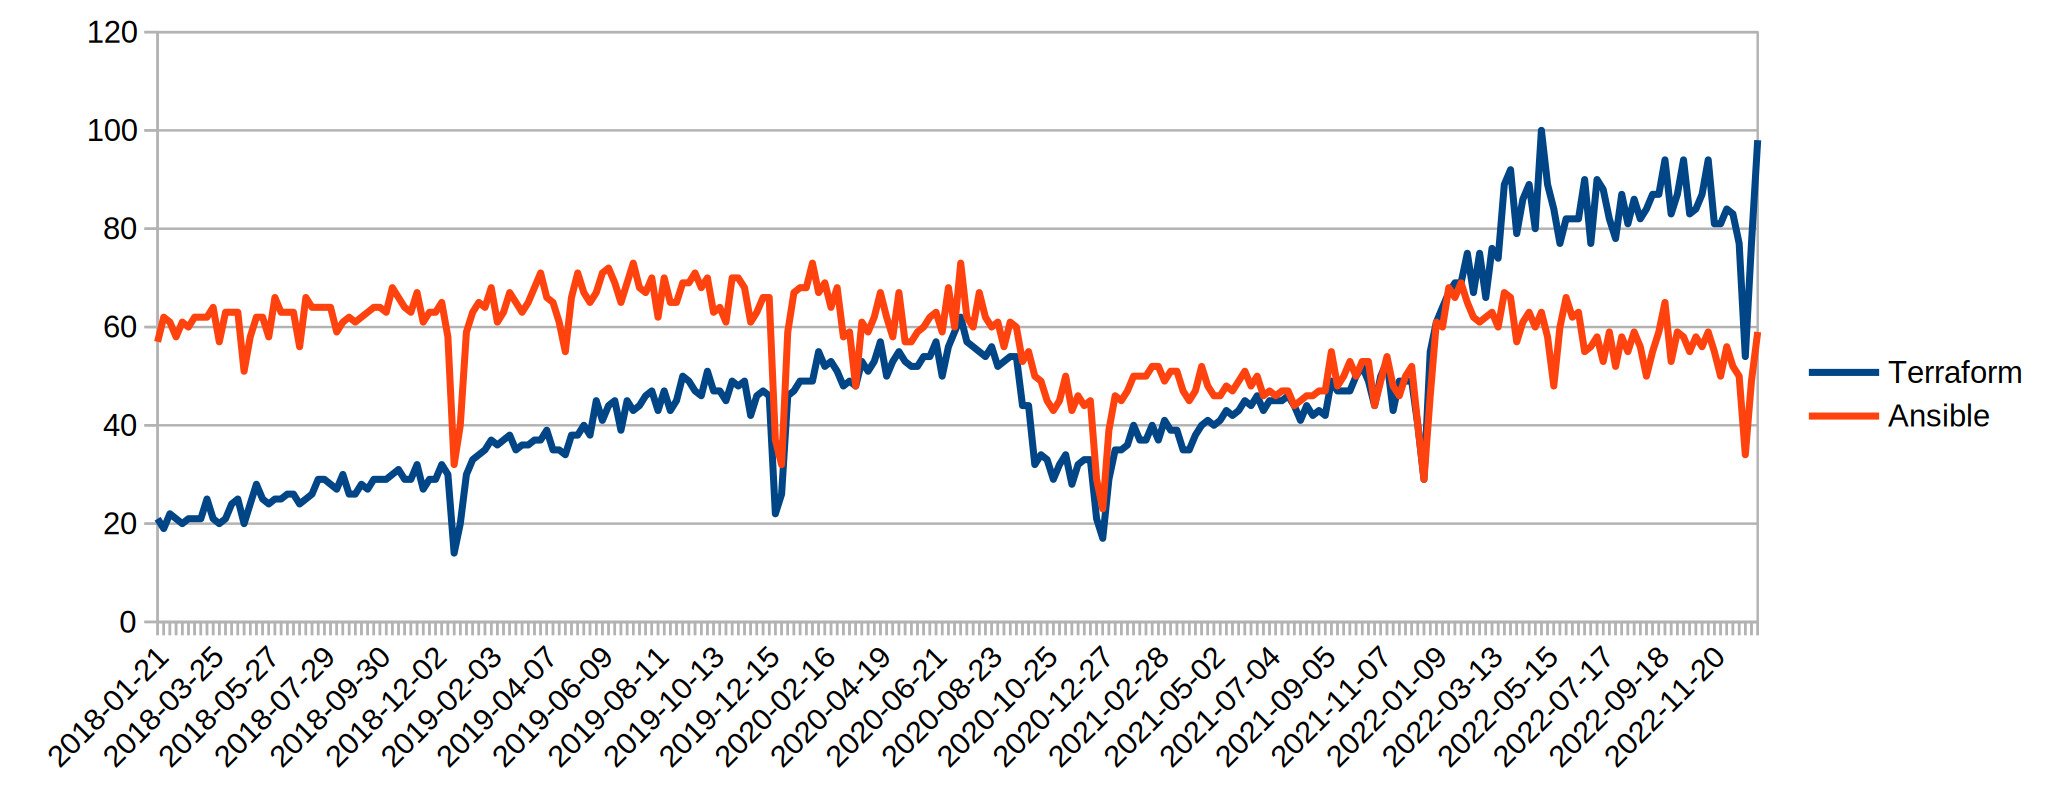
\includegraphics{../charts/trends-world.pdf}
				}
			\end{figure}
	}
	
	
	
	
	\frame{
		\frametitle{Conclusión}
			\begin{itemize}
				\footnotesize
				\item[] Cuanto mayor sea la infraestructura por aprovisionar, más evidentes serán los beneficios de Terraform, que resolverá las dependencias y optimizará el despliegue automáticamente
				\linebreak
			
				\item[] Con el tamaño crecerá la probabilidad de que haya etapas del despliegue que no sea capaz de asumir por su cuenta. La flexibilidad de Ansible lo hace una mejor herramienta para navegar los requisitos de despliegue de una aplicación, sus necesidades y su infraestructura
				\linebreak
			\end{itemize}

	}
	
	
	
	\frame{
		\frametitle{Referencias}
			\begin{itemize}
				\scriptsize
				\item[1] Hashicorp. (2023). \textit{Terraform Languague Documentation} \texttt{https://developer.hashicorp.com/terraform/language}
				\linebreak
			
				\item[2] Stack Overflow. (2022). \textit{Developer Survey 2022} \texttt{https://survey.stackoverflow.co/2022/\#most-popular-
technologies-tools-tech-prof}
				\linebreak
				
				\item[3] Google Trends. (2022). \textit{Comparación de Terraform y Ansible en los últimos 5 años} \texttt{https://trends.google.es/trends/explore?date=today\%205-y\&q=Terraform,Ansible}
				\linebreak
				
				\item[4] Google Trends. (2022). \textit{Comparación de Terraform y Ansible en los últimos 5 años} \texttt{https://trends.google.es/trends/explore?date=today\%205-y\&q=Terraform,Ansible}
				\linebreak
			\end{itemize}

	}
	
	
	
	
	
\end{document}